\documentclass[border=10pt, tikz]{standalone}
\usepackage{tikz}
\usepackage{fontspec}
\setmainfont{Times New Roman}
\setsansfont{Arial}
\usetikzlibrary{arrows.meta, positioning}

\begin{document}
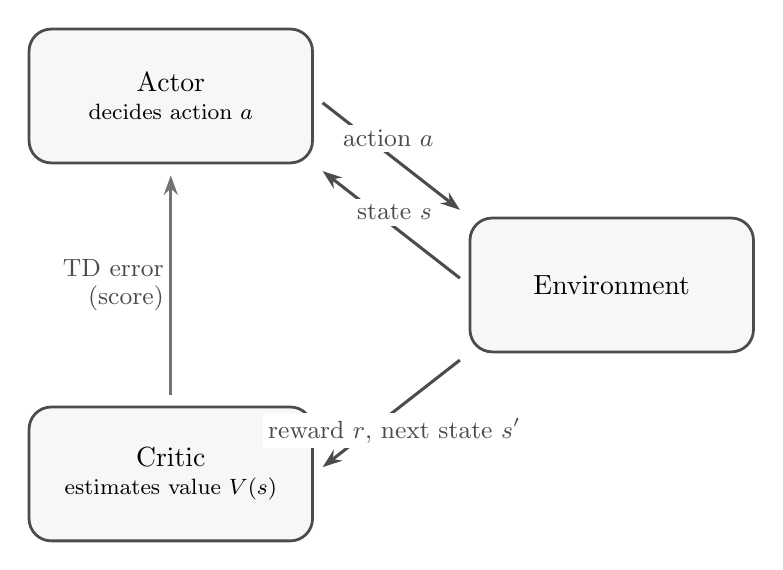
\begin{tikzpicture}[
    box/.style={
        draw=black!70, rounded corners=8pt, minimum width=3.6cm, minimum height=1.7cm,
        font=\normalsize, align=center, line width=1pt, fill=black!3
    },
    arrow/.style={
        -{Stealth[length=7pt, width=5pt]}, line width=1.1pt, black!70,
        shorten >=4pt, shorten <=4pt
    },
    feedback/.style={
        -{Stealth[length=7pt, width=5pt]}, line width=1.1pt, black!55,
        shorten >=4pt, shorten <=4pt
    },
    lbl/.style={font=\small, align=center, text=black!70, fill=white, inner sep=2pt}
]

\node[box] (actor) at (0, 2.4) {Actor\\[-2pt]{\footnotesize decides action $a$}};

\node[box] (env) at (5.6, 0) {Environment};

\node[box] (critic) at (0, -2.4) {Critic\\[-2pt]{\footnotesize estimates value $V(s)$}};

\draw[arrow] (actor.east) -- node[above, lbl, pos=0.48] {action $a$} (env.north west);

\draw[arrow] (env.west) -- node[above, lbl, pos=0.48] {state $s$} (actor.south east);

\draw[arrow] (env.south west) -- node[below, lbl, pos=0.48] {reward $r$, next state $s'$} (critic.east);

\draw[feedback] (critic.north) -- node[left, lbl, align=right] {TD error\\[-1pt](score)} (actor.south);

\end{tikzpicture}
\end{document}
